\chapter{Astroteilchenphysik}
\label{chapter:Astroteilchenphysik}
Das Gebiet der Astroteilchenphysik ist noch ein recht junges Gebiet der Physik und beschäftigt sich mit einer Kombination aus Astrophysik und Teilchenphysik.
Verschiedene Botenteilchen, deren Vor- und Nachteile in \autoref{sec:KosmischeStrahlung} beschrieben werden, geben Auskünfte über Quellen (siehe \autoref{sec:Quellen}).
Die Energie dieser in den Quellen beschleunigten Teilchen übersteigt zum Teil die höchste Energie, die auf der Erde mit Beschleunigern erreicht werden kann.
Die Modelle für die grundlegenden Beschleunigungsmechanismen (siehe \autoref{sec:Beschleunigungsmechanismen}) müssen noch überprüft, bzw. weiterentwickelt werden.
Im Verlauf der Jahre haben sich verschiedene Detektionsarten entwickelt und sind speziell angepasst an die Teilchen, die detektiert werden.
Dabei ist die Forschung in der Detektorentwicklung noch nicht am Ende und die Kollaborationen, sowie die konzipierten Detektoren werden größer.
Beispiele dafür ist der Icecube-Neutrino-Detektor oder das geplante Cherenkov-Teleskop-Array CTA.
\autoref{sec:Gammaastronomie} bietet eine Übersicht über die Gammaastronomie und beschreibt die Wechselwirkung der Photonen auf dem Weg von der Quelle zum Detektor. 
Im \autoref{sec:AGN} wird noch einmal der spezielle Quelltyp des Aktiven Galaktischen Kerns [Active Galctic Nuclei (AGN)] näher beschrieben.
Der letzte Abschnitt - \autoref{sec:Mrk421} - bietet eine Übersicht über die AGN Mrk 421, die im Verlauf der Arbeit analysiert wird.

\section{Kosmische Strahlung}
\label{sec:KosmischeStrahlung}

\begin{figure}
    \centering
    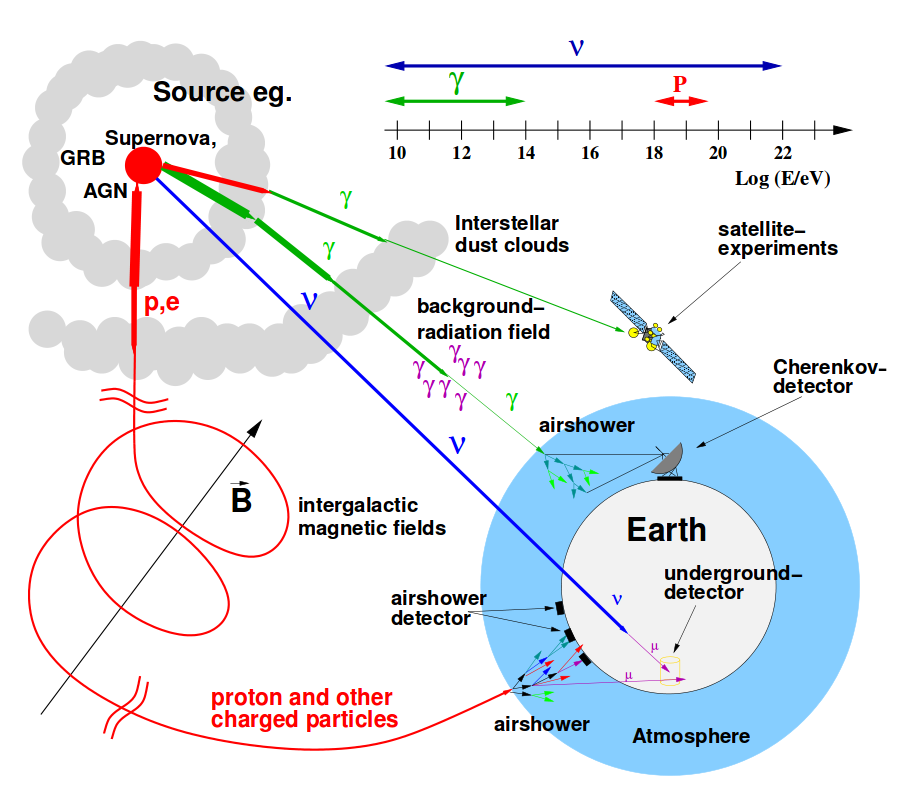
\includegraphics[width=0.8\textwidth]{./Plots/02_Astroteilchenphysik/Astroteilchen.png}
    \caption{Auf dem Weg von der Quelle zum Beobachter unterliegen die unterschiedlichen Botenteilchen unterschiedlichen Wechselwirkungen. 
    Geladene Teilchen wechselwirken mit Staubwolken und werden von Magnetfeldern abgelenkt, Neutrinos und hochenergetische Photonen behalten ihre Richtungsinformation bei.
    Photonen wechselwirken ebenfalls mit Staubwolken oder mit niederenergetischen Hintergrundphotonen und werden dann abhängig von ihrer Energie mit unterschiedlichen Detektoren detektiert. 
    Das Bild entstammt \cite{DissMarlene}.}
    \label{Astroteilchen}
\end{figure}


\autoref{Astroteilchen} zeigt eine schematische Darstellung der verschiedenen Botenteilchen, die von einer astrophysikalischen Quelle emittiert werden können.

Geladene Teilchen wie z.B. Protonen oder Elektronen werden aufgrund ihrer Ladung auf ihrem Weg von der Quelle zum Beobachter von Magnetfeldern abgelenkt und verlieren damit ihre Richtungsinformationen.

Neutrinos hingegen können wegen ihrer geringen Wechselwirkungswahrscheinlichkeit diese Strecke ungehindert zurücklegen. 
Allerdings ist ihre Detektion schwierig.
Detektoren mit großem Volumen können sie indirekt z.B. über Myonen detektieren.

Hochenergetische Photonen besitzen den gleichen Vorteil wie Neutrinos und werden auf dem Weg zum Detektor nicht abgelenkt.
Allerdings wechselwirken sie mit Staubwolken oder Hintergrundphotonen, sodass sie abhängig von ihrer Energie mit Satellitenexperimenten direkt oder über Luftschauerteleskope indirekt detektiert werden können.

\subsection{Geladene kosmische Strahlung}
Die geladene kosmische Strahlung wurde Anfang des 20. Jahrhunderts mit Hilfe von Ballonexperimenten entdeckt \cite{Hess}.
Aufgrund der Tatsache, dass mit steigender Höhe die Ionisation zunahm, schlossen Hess und Kohlhörster, dass die von ihnen detektierte Strahlung aus dem Weltraum kommen müsse. \cite{Kohlhoerster}
Diese Strahlung besteht zu 85\% aus Protonen, zu 12\% aus $\alpha$-Teilchen und 3\% aus Elementen mit größerer Kernladung.\cite{Grupen}
Das Energiespektrum dieser kosmischen Strahlung ist auf einem sehr großen Energiebereich bekannt und wurde sowohl mit erdgebundenen als auch mit Satellitenexperimenten bestimmt.


\begin{figure}
    \centering
    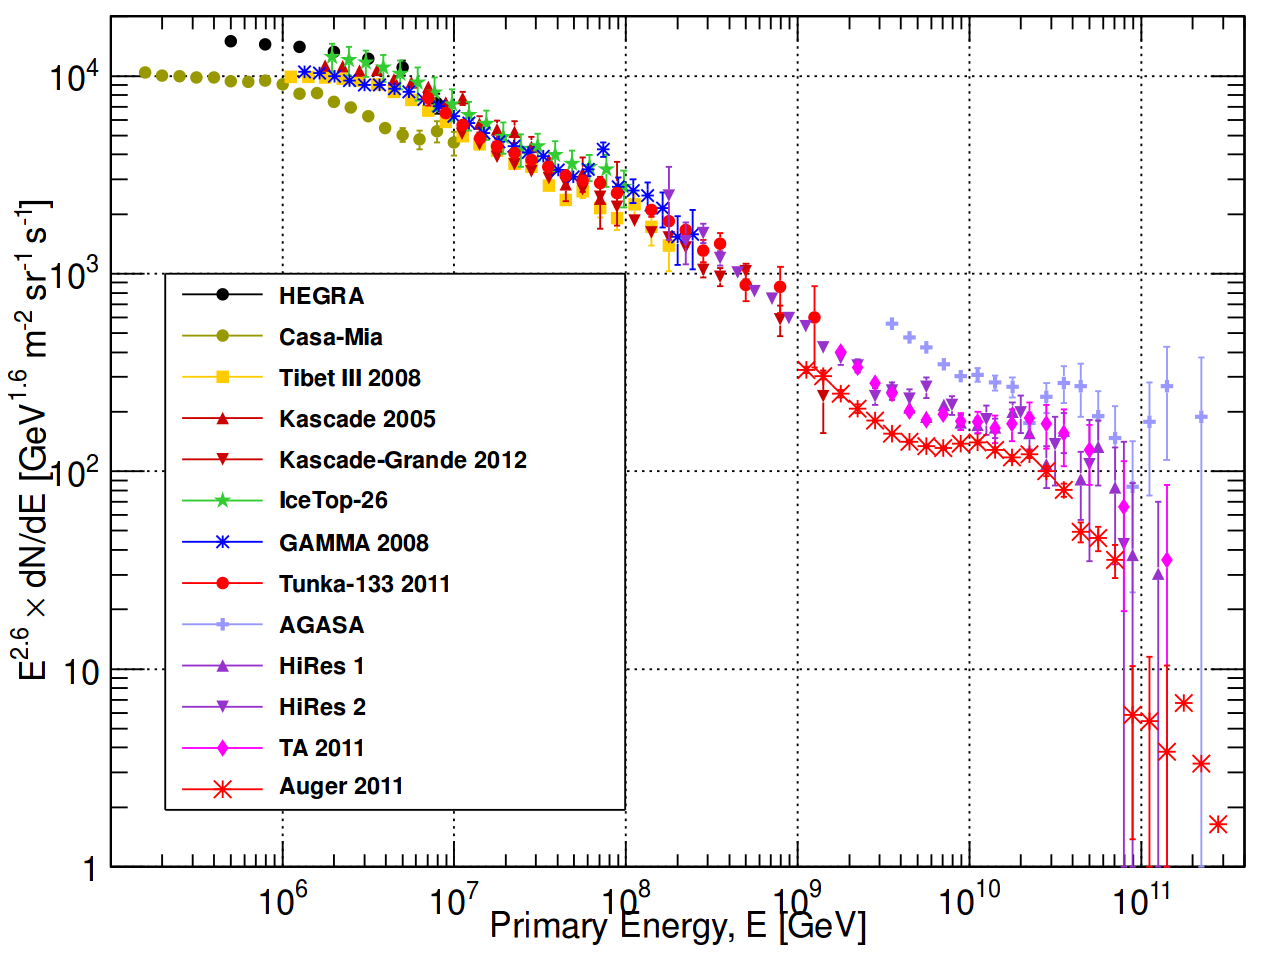
\includegraphics[width=0.8\textwidth]{./Plots/02_Astroteilchenphysik/CosmicRaySpectrum.png}
    \caption{Spektrum der kosmischen Strahlung: Bei der Energie $E=10^{6.4}\,\si{GeV}$ befindet sich das sogenannte "Knie" und bei der Energie $E=10^{9.5}\,\si{GeV}$ die "Ferse" des Spektrums. \cite{GaisserSpektrum}}
    \label{CR-Spektrum}
\end{figure}



Wie in \autoref{CR-Spektrum} zu erkennen ist, kann das Spektrum mit einem gebrochenen Potenzgesetz mit zwei Steigungsänderungen, die als "Knie" und "Ferse" bezeichnet werden, beschrieben werden \cite{DissBecker}:

\begin{equation}
 \frac{dN}{dE_{CR}} \propto E_p^{-\alpha_{CR}}
\end{equation}

mit 

\begin{equation*}
\alpha_{CR}=	
\left\{
\begin{aligned}
2,67 \qquad \log\left( \frac{E_{CR}}{eV} \right) &< 15,4 \\
3,10 \qquad \log\left( \frac{E_{CR}}{eV} \right) &< 18,5 \\ 
2,75 \qquad \log\left( \frac{E_{CR}}{eV} \right) &> 18,5.
\end{aligned}
\right.
\end{equation*}

Größere Energien als $5 \cdot 10^{19} \si{eV}$ können aufgrund des GZK-Cutoffs \cite{Greisen}\cite{ZatsepinKuzmin} nicht gemessen werden. 
Dieser Cutoff tritt auf, wenn Protonen mit dem kosmischen Mikrowellenhintergrund (CMB) wechselwirken \cite{DissBecker}: 

\begin{equation*}
p\gamma_{CMB}=	
\left\{
\begin{aligned}
& \Delta^+ \\
& p e^+ e^- .
\end{aligned}
\right.
\end{equation*}

Knie und Ferse beinhalten Informationen über die Beschleunigungsmechanismen der Teilchen, bzw. über die Quellen.
Die Teilchen mit den höchsten Energien, jenseits der Ferse können nicht galaktischen Ursprungs sein, da die galaktischen Magnetfelder für die Beschleunigung zu schwach sind. 
Deswegen wird vermutet, dass diese Teilchen extragalaktischen Ursprungs sind, wobei die Beschleunigungsmechanismen (vgl. \autoref{sec:Beschleunigungsmechanismen}) noch nicht genau bekannt sind.

\subsection{Neutrinos}
Neutrinos sind leichte Teilchen, die eine sehr geringe Wechselwirkungsqahrscheinlichkeit haben und so in großen Experimenten wie IceCube\cite{Icecube} oder ANTARES\cite{ANTARES} indirekt über Myonen nachgewiesen werden.
Das größte Problem bei der Suche nach hochenergetischen Neutrinos ist der Untergrund, der in Wechselwirkungen von geladener kosmischer Strahlung in der Atmosphäre entsteht.
Neutrinos werden in hadronischen Reaktionen erzeugt und können auf dem Weg von der Quelle zum Detektor oszillieren.
Die Produktion von Neutrinos geschieht über die Produktion von geladenen Pionen und folgende Reaktionen sind möglich:
Entweder wechselwirkt ein Photon mit einem Proton folgendermaßen mit der angegebenen Wahrscheinlichkeit\cite{DissBecker}:

\begin{equation*}
p\gamma \rightarrow \Delta^+ \rightarrow	
\left\{
\begin{aligned}
& p \pi^0 \qquad [2/3] \\
& n \pi^+ \qquad [1/3]
\end{aligned}
\right.
\end{equation*}

oder ein Proton wechselwirkt mit einem anderen Proton\cite{DissBecker}:

\begin{equation*}
p p \rightarrow
\left\{
\begin{aligned}
& p p \pi^0 \qquad [2/3] \\
& p n \pi^+ \qquad [1/3].
\end{aligned}
\right.
\end{equation*}

Die gleichen Prozesse treten auch für Neutronen oder bei höheren Energien Kaonen als Primärteilchen auf, wodurch negativ geladene Pionen entstehen.
Die Pionen zerfallen dann und erzeugen weitere Neutrinos \cite{DissBecker}:

\begin{equation*}
 \begin{aligned}
 \pi^+ \rightarrow \mu^+ \nu_{\mu} \rightarrow e^+ \nu_e \overline{\nu}_{\mu} \nu_{\mu} \\ 
 \pi^- \rightarrow \mu^- \overline{\nu}_{\mu} \rightarrow e^- \overline{\nu}_e \nu_{\mu} \overline{\nu}_{\mu}
 \end{aligned}
\end{equation*}

Aufgrund der beschriebenen Prozesse erwartet man in der Quelle eine Verteilung der Neutrinos von $(\nu_e:\nu_{\mu}:\nu_{\tau})=(\overline{\nu}_e:\overline{\nu}_{\mu}:\overline{\nu}_{\tau})=(1:2:0)$.
Propagieren die Neutrinos Strecken von der Größenordnung des Sonnensystems, oszillieren sie, sodass auf der Erde ein Verhältnis von $(\nu_e:\nu_{\mu}:\nu_{\tau})=(1:1:1)$ beobachtet wird.

Es gibt verschiedene Neutrinoquellen:
\begin{itemize}
 \item Kosmogene Neutrinos werden in Wechselwirkungen von hochenergetischen Protonen mit dem CMB und den darauffolgenden Zerfall von geladenen Pionen erzeugt.
 \item Galaktische Neutrinos können in hadronischen Beschleunigungsprozessen erzeugt werden.
 \item Es wird erwartet, dass in Gamma Ray Bursts Neutrinos erzeugt werden.
 \item In den hadronischen Modellen von AGNs werden Neutrinos produziert. 
\end{itemize}

\subsection{Photonen}
Genau wie die Neutrinos haben Photonen den Vorteil, dass sie nicht von Magnetfeldern abgelenkt werden.
Allerdings könenn aufgrund der Absorption in der Atmosphäre auf der Erde nur Photonen im optischen und im Radiobereich detektiert werden.
Deswegen wurden diese Wellenlängen in der Astronomie auch als erstes benutzt. 
Nach und nach kamen dann die anderen Wellenlängen wie z.B. Röntgenstrahlung oder Gammastrahlung hinzu.
Gammastrahlung lässt sich anhand der Energie in nieder- bis mittelenergetische Gammastrahlung ($\SI{0,1}{MeV}$ - $\SI{30}{MeV}$), hochenergetische Gammastrahlung ($\SI{30}{MeV}$ -$\SI{100}{GeV}$), sehr hochenergetische Gammastrahlung ($\SI{100}{GeV}$-$\SI{100}{TeV}$) und ultrahochenergetische Gammastrahlung ($E>\SI{100}{TeV}$) einteilen.
Der Energiebereich bis ca. 100GeV lässt sich nur mit Satellitenexperimente nachweisen.
Die sehr hochenergetische und die ultrahochenergetische Strahlung lässt sich wiederum mit Hilfe von Luftschauerteleskopen auf der Erde detektieren.\cite{Weekes}

Das Problem der hochenergetischen Photonen ist, dass sie mit den niederenergetischen Photonen der Hintergrundstrahlung (EBL) wechselwirken.
Mit Hilfe von Modellen kann die Absorption von hochenergetischen Photonen aus extragalaktischen Quellen durch diese Hintergrundstrahlung berechnet werden.\cite{Weekes}

In \autoref{sec:Gammaastronomie} wird dann noch näher auf die Gammaastronomie eingegangen und es werden die Wechselwirkungen erklärt, die die Photonen auf ihrem Weg zur Erde, erfahren.


\section{Quellen kosmischer Strahlung}
\label{sec:Quellen}
In diesem Kapitel wird eine Übersicht über die Quellen der kosmischen Strahlung gegeben.

\subsection{Die Galaktische Scheibe und das Galaktische Zentrum}
Die galaktische Scheibe ist die stärkste und erste detektierte Gammaquelle und wurde 1968\cite{GalacticPlane} detektiert.
Im Folgenden werden die Prozesse beschrieben, die die galaktische Gammastrahlung erzeugen:

\begin{itemize}
 \item Kosmische Elektronen erzeugen niederenergetische Photonen durch Bremsstrahlung mit dem Interstellaren Gas.
 \item Hadronen der kosmischen Strahlung produzieren neutrale Pionen, die dann in zwei Photonen mit mittlerer Energie zerfallen.
 \item Kosmische Elektronen überleben eine inverse Comptonstreuung an niederenergetischen Gammaphotonen und erzeugen Photonen mit hohen Energien.
\end{itemize}

Das Galaktische Zentrum enthält mehrere Objekte, wie z.B. junge Supernova-Remnants wie Sgr $A$ East, die hochenergetische Gammastrahlen emittieren.
Das dynamische Zentrum wurde mit der kompakten Radioquelle Sgr $A^*$ assoziiert, welche vermutlich ein supermassives schwarzes Loch ist.
In einem Radius von 10pc um das Galaktische Zentrum befindet sich eine Masse von $3\cdot 10^7$ Sonnenmassen.
Das Satellitenexperiment EGRET hat die Quelle 3EG J1745-2852 detektiert, welche hochenergetische Gammastrahlung emittiert. 
Die Natur dieser Quelle ist noch unbekannt.\cite{GalacticCenter}\cite{Weekes}


\subsection{Supernovae und Supernovaremnants}
Die Explosion eines Sterns wird als Supernova (SN) bezeichnet.
Gammastrahlung, die aus SN kommt, wird entweder in den ersten Sekunden der Explosion als Gammastrahlenausbruch [Gamma Ray Burst (GRB)] detektiert oder als stete periodische Emission des entstandenen Pulsars.
Es ist auch möglich, dass sie der sich ausbreitenden Hülle des ehemaligen Sterns [Supernova Remnant (SNR)] entstammen. 
Diese galktischen Quellen liefern kosmische Strahlung bis zu Energien von $\SI{100}{TeV}$.
SN und SNR vermögen es nicht, Teilchen auf Energien von $10^20\,\si{eV}$ zu beschleunigen.
Somit entstammen Teilchen mit so hohen Energien extragalaktischen Quellen.\cite{Weekes}

Die Beschleunigung der Teilchen erfolgt in Schockwellen.
Das Modell dieser diffusen Schockbeschleunigung liefert ein Potenzgesetz für das Spektrum der beschleunigten Strahlung von $\frac{dN}{dE} \propto E^{-2,0}$.
Dieses Potenzgesetz wird um Effekte während der Propagation durch die Galaxie korrigiert und resultiert in einem Spektrum der kosmischen Strahlung von $\frac{dN}{dE} \propto E^{-2,7}$
Im Allgemeinen sind die Spektra von Supernovae hart und haben einen Cutoff bei ca. $\SI{20}{TeV}$, was auf eine Primärteilchenenergie von einigen TeV schließen lässt.\cite{Weekes}\cite{RhodeFalke}


\subsection{Gamma Ray Pulsars und Binaries}
Pulsare sind rotierende Neutronensterne. 
Das bekannteste Beispiel ist der Crab Pulsar im Zentrum des Krebsnebels.
Dieser Quelltyp wurde vor mehr als 30 Jahren entdeckt und er lässt sich in zwei Kategorien einteilen.
Der erste Typ gewinnt seine Energie durch Rotation und ist im Radiobereich detektierbar und der andere Quelltyp gewinnt seine Energie durch Akkretion von Materie und ist im Röntgenbereich detektierbar.
Pulsare haben Rotationsperioden zwischen einigen Millisekunden und einigen Sekunden.
Vor allem im Gammabereich ist ihre Luminosität hoch und genau wie bei den SN und SNRs können ihre Energiespektren durch ein Potenzgesetz beschrieben werden.
Verschiedene Pulsare lassen sich anhand ihrer Spektren voneinander unterschieden; auch unterscheiden sich ihre Lichtkurven in der Position der Peaks bei verschiedenen Wellenlängen.
Die Theorie von Pulsaren ist noch nicht komplett verstanden, weswegen Modelle getestet werden.\cite{Weekes}

Die Hälfte aller Sterne taucht in einer Assoziation mit einem anderen Objekt auf und wird Binaries genannt.
Dieses andere Objekt ist oft ein kompaktes Objekt wie ein Weißer Zwerg, ein Neutronenstern oder ein Schwarzes Loch.
Hohe Röntgenemission sowie ein zeitlich variables Verhalten sind charakteristisch für diesen Quelltyp.
Dabei kann die Variabilität im Bereich von Millisekunden bis zu Jahren liegen und periodisch auftauchen oder in einzelnen Ausbrüchen, Flares genannt.\cite{Weekes}


\subsection{Gamma Ray Bursts}
Gammastrahlenausbrüche (GRBs) wurden während des kalten Kriegs von den amerikanischen Vela-Satelliten, die Atombombenexplosionen aufspüren sollten, entdeckt.
16 GRBs mit Zeitspannen von $\SI{0,1}{s}$-$\SI{30}{s}$ mit Flüssen zwischen $(10^{-5}-10^{-4}\,\frac{\si{erg}}{\si{s}}$ wurden detektiert.
Allgemein dauern GRBs zwischen Millisekunden und einigen tausend Sekunden und sind isotrop verteilt.
Sie werden in kurzzeitige Bursts ($t<\SI{2}{s}$) und den Rest unterteilt.
Fast die gesamte emittierte Energie ist größer als $\SI{50}{keV}$.
Mit Satellitenexperimenten wurden GRBs auch im Gammabereich (bis ca. $\SI{30}{GeV}$) detektiert, der Fluss ist aber sehr niedrig.
Bodengebundene Teleskope, wie z.B. MAGIC haben GRB-Programme, allerdings kam es bisher noch zu keiner richtigen Detektion.\cite{Weekes}


\subsection{Aktive Galaktische Kerne}
Die Klasse der Aktiven Galaktische Kerne (AGN) wird durch ein supermassives schwarzes Loch, welches sich in ihrem Zentrum befindet und Materie akkretiert, gekennzeichnet. 
Anhand ihrer Ausrichtung zum Beobachter und ihrer Emission in den verschiedenen Wellenlängen werden AGNs klassifiziert. 
Eine genauere Darstellung dieses Quelltyps, zu dem auch die in dieser Arbeit analysierte Quelle gehört, wird in \autoref{sec:AGN} gegeben.

\section{Beschleunigungsmechanismen} 
\label{sec:Beschleunigungsmechanismen}
Im Folgenden werden die Beschleunigungsmechanismen vorgestellt, die in den relativsitischen Jets von AGNs oder GRBs relevant sind.
Dafür wird zunächst der Fermi-Mechanismus vorgestellt, mit Hilfe dessen geladenen Teilchen beschleunigt wird.
Danach werden die Prozesse zur Erzeugung, bzw. Abschwächung von hochenergetischer Gammastrahlung beschrieben.
Wegen der geringen Teilchendichte in Jets ($n\leq 10^{-3}\,\frac{1}{cm^3}$) werden Prozesse wie Coulombstreuung oder Bremsstrahlung nicht beschrieben.

\subsection{Fermi-Mechanismus 1. und 2. Art}
Die Fermi-Beschleunigung 1.Art beschreibt die Schockbeschleunigung.
Die in einer SN abgestoßene Hülle repräsentiert eine Schockfront, die sich mit einer Geschwindigkeit $u_1$ durch das Interstellare Medium (ISM) fortbewegt. 
Dahinter strömt das Gas mit einer Geschwindigkeit $u_2$ weg.
Kollidiert nun ein Teilchen, welches sich mit der Geschwindigkeit $c$ bewegt, mit dieser Schockfront und wird dabei reflektiert, so gewinnt es die Energie

\begin{equation}
 \frac{\Delta E}{E}\propto \frac{u_1-u_2}{c}.
\end{equation}

Diese Art der Beschleunigung ist somit linear in der Geschwindigkeit und es können maximale Energien von $\approx 100\si{TeV}$ erreicht werden.\cite{Grupen}\cite{Longair}

Die Fermi-Beschleunigung 2.Art beschreibt die Wechselwirkung eines Teilchens mit Geschwindigkeit c mit magnetischen Gaswolken, die sich mit der Geschwindigkeit u bewegen:

\begin{equation}
 \frac{\Delta E}{E}\propto \frac{u^2}{c^2}.
\end{equation}

Die Fermi-Beschleunigung 2.Art ist somit quadratisch in der Wolkengeschwindigkeit.
Da die Teilchen der kosmischen Strahlung einen Teil ihrer Energie in Wechselwirkungen mit dem interstellaren oder dem intergalaktischen Gas zwischen zwei Kollisioinen wieder verlieren, benötigt dieser Beschleunigungsmechanismus eine minimale Injektionsenergie, oberhalb der Teilchen effektiv beschleunigt werden können.\cite{Grupen}\cite{Longair}


\subsection{Synchrotronstrahlung}
Fliegt ein geladenes relativistisches Teilchen durch ein Magnetfeld, emittiert es ein breites Spektrum an Synchrotronstrahlung.
Der Energieverlust dieses Teilchens mit Masse m, Ladung q, Lorentzfaktor $\gamma$ und der Geschwindigkeit $\beta c$, welches sich mit einem Winkel $\Psi$ zum B-Feld mit der Energiedichte $u_B=\frac{B^2}{8\pi}$ bewegt beträgt:

\begin{equation}
 \left( \frac{dE}{dt} \right)_{Sy} = - \frac{16 \pi c}{3} \left(\frac{q}{mc^2} \right)^2 u_B \beta^2 \gamma^2 sin^2(\Psi).
\end{equation}

Unter der Annahme, dass in relativistischen Jets die abstrahlenden Teilchen sofort in zufällige Richtungen gestreut werden, d.h. dass sie zufällig im Verhältnis zum B-Feld verteilt sind und unter der Annahme, dass die Streuung auf kleineren Zeitskalen als die Synchrotronstrahlung passiert, wird über den Winkel $\psi$ gemittelt.
Das führt dazu, dass der Energieverlust umso größer wird, je größer die Masse ist:

\begin{equation}
 \frac{dE}{dt}\propto m^{-2}, \qquad \text{bzw.} \qquad \frac{d\gamma}{dt}\propto m^{-3}.
\end{equation}

Daraus folgt, dass Elektronen ihre Energie effizienter durch Synchrotronstrahlung verlieren können als Protonen.
Für den gleichen Energieverlust müsste ein Proton $6,2 \cdot 10^9$ mal mehr Energie haben.
Das Problem von Elektronen ist, dass sie nachdem sie zu ultrarelativistischen Energien beschleunigt worden sind, ihre Energie sehr schnell wieder verlieren.
Protonen und schwerere Teilchen können einfacher beschleunigt werden,  müssen aber auf extrem hohe Energien beschleunigt werden, um Photonen mit nennenswerter Energie abstrahlen zu können.

Zudem tritt noch das Problem der Synchrotron-Selbst-Absorption auf, d.h. Photonen werden von relativistischen Elektronen im B-Feld absorbiert.\cite{RelativisticJets}

\subsection{Compton-Streuung}
Die Streuung von relativistischen Elektronen an einem Strahlungsfeldes in extragalaktischen Jets wird Compton-Streuung genannt.
Die Photonenergie wird in Abhängigkeit von der Elektron Ruhe-Masse $m_e c^2$ angegeben: $\epsilon= \frac{h\nu}{m_e c^2}$.\cite{RelativisticJets}
 
In niedrigster Ordnung ist der Energieverlust im Thomson Limit, d.h. $\gamma \epsilon <<1$ gegeben durch:

\begin{equation}
-\left(\frac{d\gamma}{dt} \right) \approx \frac{4}{3} c \sigma_T \frac{u_{ph}}{m_e c^2} \gamma^2
\end{equation}

\begin{center}
 \begin{tiny}
  $\sigma_T$: Thompson-Wirkungsquerschnitt, $u_{Ph}$: Energiedichte des Photonfeldes.
 \end{tiny}
\end{center}

Im Thompson-Limit kommt es zu Photonenergien von $\epsilon_S ~\gamma^2 \epsilon_0 << \frac{1}{\epsilon_0} $, wobei $\epsilon_0$ die Energie des isotropen monoenergetischen Photonfeldes ist.\cite{RelativisticJets}

Für große Elektron- und Photonenergien $\gamma \epsilon > 1$ ist Compton-Streuung unterdrückt.\cite{RelativisticJets}


\subsection{$\gamma\gamma$-Absorption und Paar-Produktion}
Die Wechselwirkung von hochenergetischen Photonen miteinander oder mit weniger energiereichen Photonen ist der einzige relevante Absorptionsmechanismus für Photonen in astrophysikalischen Umgebungen.
Ein Photon mit der Energie $\epsilon_1$ wechselwirkt mit einem Photon mit der Energie $\epsilon_2$ unter dem Winkel $\Theta=cos^{-1}\mu$ und produziert ein $e^+/e^-$-Paar falls:
\begin{equation}
 \epsilon_1 \geq \frac{2}{\epsilon_2 (1-\mu)}.
\end{equation}

VHE-Gammastrahlung aus einer Quelle in kosmologischer Entfernungen wird vom Infrarot- und optischen Hintergrundlicht absorbiert. 
Dieser Prozess wird EBL (Extragalactic Background Light)-Absorption genannt. 
Dieses extragalaktische Hintergrundlicht besteht vorwiegend aus der Infrarot-Emission von Staub aus jungen, sternbildenden Galaxien als auch aus der Infrarot- und der optischen Emission von Sternen.
Das Spektrum und die Intensität des EBL hängen von der kosmologischen Zeit bzw. der Rotverschiebung ab und dadurch wird auch die Opazität für VHE-Gammastrahlung bestimmt.
Wegen der großen Emission innerhalb des Sonnensystems und der Milchstraße ist der EBL schwierig zu vermessen.\cite{RelativisticJets}


\subsection{$\gamma$-Hadron-Wechselwirkungen}
Aufgrund der oft dichten Strahlungsfelder in Jets sind die Wechselwirkungen zwischen relativistischen Hadronen und Photonen wichtig.
Zum einen kann es zu Bethe-Heitler-Paarproduktion und zum anderen zu Photomesonproduktion kommen.\cite{RelativisticJets}

Die Bethe-Heitler-Paarproduktion beschreibt die Reaktion eines Kernteilchens an einem Hintergrund-Photon, wobei ein $e^+/e^-$-Paar entsteht:
\begin{equation}
 p \gamma \rightarrow p' e^+ e^-.
\end{equation}

Diese Reaktion tritt auf, sobald die Schwerpunktsenergie groß genug ist:
\begin{equation}
 s \geq (m_p c^2 +2 m_e c^2)^2 \approx 0,882\si{GeV^2}.
\end{equation}

Die Photomesonproduktion von z.B. Pionen tritt auf, sobald die Schwerpunktsenergie $s \geq (m_p c^2 +2 m_{\pi^0} c^2)^2 \approx \SI{1,16}{GeV^2}$ überschreitet.
Dominant ist die Pion-Produktion in photohadronischen Interaktionen, wobei die $\pi^0$ mit einer Halbwertszeit von $t_{1/2}\approx 8,4\cdot 10^{-17}\,\si{s}$ in zwei Photonen zerfallen und die geladenen Pionen nach einer Halbwertszeit von $t_{1/2}\approx 2,6\cdot 10^{-8}\,\si{s}$ in Myonen und Neutrinos.
Die Produktion und der Zerfall von Kaonen und $\eta$-Mesonen trägt (10-20)\% zur gesamten Photonen-, Leptonen- und Neutrinoproduktion bei.\cite{RelativisticJets}

\subsection{Photodisintegration}
Für Protonen ist der Verlust durch Photomesonproduktion dominierend gegenüber der Bethe-Heitler-Paarproduktion. 
Photodisintegration ist vernachlässigbar.
Photodisintegration beschreibt die Anregung eines Kerns durch ein Photon.
Bei der Abregung wird ein ein oder mehrere Protonen oder Neutronen oder Alpha-Teilchen sowie ein oder mehrere Photonen.
Der Wirkungsquerschnitt hat eine Resonanz ("giant dipole resonance") der Höhe $\sigma_{A\gamma}\approx A \si{mb}$.\cite{RelativisticJets}

\subsection{Elektromagnetische Kaskaden}
In einer photohadronischen Quelle ist die Lichtundurchlässigkeit für primäre Gammastrahlung aus $\pi^0$-Zerfällen oder Compton-Streuung groß, weil sonst keine photohadronischen Wechselwirkungen stattfinden würden.
Solche primären Photonen verursachen eine elektromagnetische Kaskade aus Paarproduktion, Synchrotronstrahlung, Comptonstreuung und Bremsstrahlung.
Dieser Prozess kann innerhalb Jets auftreten, sobald die Photonen genug Energie für die Paarproduktion besitzen und die Dichte an Umgebungsphotonen hoch genug ist.
Sobald die Energie der Photonen nicht mehr ausreichend für die Paarproduktion ist, verschwindet die Kaskade.\cite{RelativisticJets}


\section{Gammaastronomie}
\label{sec:Gammaastronomie}


\begin{figure}
    \centering
    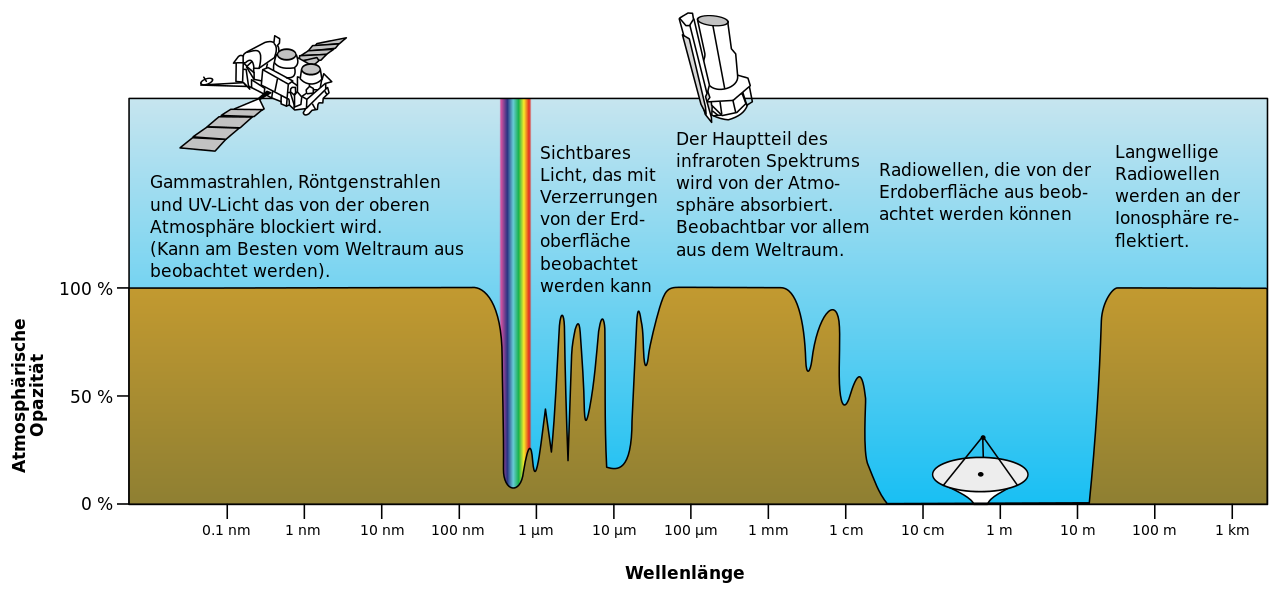
\includegraphics[width=0.99\textwidth]{./Plots/02_Astroteilchenphysik/Atmospheric_electromagnetic_opacity.png}
    \caption{Zu sehen ist die Durchlässigkeit der Atmosphäre für elektromagnetische Strahlung in Abhängigkeit von der Wellenlänge.\cite{Opazitaet}}
    \label{EM-Opazitaet}
\end{figure}


Wie in \autoref{EM-Opazitaet} zeigt, ist die Atmosphäre transparent für optische Beobachtungen und Radiowellen. 
Alle anderen Wellenlängen werden von der Atmosphäre geblockt, sodass bis 1960 nur in diesen Wellenlängen beobachtet wurde.
Mit der Entwicklung der Raumfahrt konnten dann auch Satellitenexperimente konzipiert werden, mit denen Gammaastronomie betrieben wurde.
Aber auch mit bodengebundenen Experimenten wird Gammaastronomie betrieben mit Hilfe von Sekundärprodukten, die mit der Atmosphäre wechselwirken.
Die minimale Energie, bei der Gammastrahlung auf der Erde detektiert werden kann ist zufällig genau über der maximalen Energie, die von Satellitenexperimenten beobachtet wird.
Die bodenegebundenen Experimente beruhen auf der Detektion des Cherenkovlichts von elektromagnetischen Schauern in der Atmosphäre.\cite{Weekes}

Die bevorzugte Wechselwirkung eines Gammateilchen, das mit einer Energie $E>\SI{10}{MeV}$ in die Atmosphäre eintritt, ist die Paaarproduktion, die meist nach einer durchlaufenen Strecke von ca. $\SI{20}{km}$ auftritt.
Das produzierte $e^+/e^-$-Paar fliegt in die gleiche Richtung wie das primäre Photon und wechselwirkt mit den Molekülen der Atmosphäre.
Dabei werden Bremsstrahlungsphotonen emittiert, die dann eine weitere Paarproduktion auslösen können.
Die resultierende Kaskade ist relativ schmal und bewegt sich in die gleiche Richtung wie das Ursprungsteilchen.
Sie wächst so lange bis die Energie der geladenen Teilchen so gering ist, dass Ionisationsverluste und Strahlungsverluste gleich groß sind und erreicht da ihr Schauermaximum.
Danach nimmt die Anzahl der Teilchen der Kaskade ab und der Schauer stirbt aus, was meistens über dem Erdboden passiert.
Die sekundären geladenen Teilchen im Schauer emittieren Cherenkovlicht in Vorwärtsrichtung unter einem Winkel von ca. 1,3°, welches dann von den Teleskopen detektiert wird.
Nicht nur primäre Photonen können solch einen Schauer induzieren, sondern auch Hadronen, wobei der Schauer kein rein elektromagnetischer ist. 
Ein hadronischer Schauer unterscheidet sich in seiner Form von einem elektromagnetischen (siehe \todo{CORSIKA-Referenz}).\cite{Weekes}

Für die Detektion wird ein Detektor mit schneller Elektronik benötigt, mit dem Ziel den Ursprung des Schauers, die Energie und die Ankunftszeit zu bestimmen.
Die Photonenanzahl im Schauer ist ein gutes Maß für die Energie des ursprünglichen Photons.
Für eine große Sensitivität muss die Lichtsammelfläche eines Telskops möglichst groß sein. 
Die Entwicklung von Teleskopen mit segmentierten Spiegeln begann mit dem Whipple-Teleskop\cite{Whipple}.
Heute nutzen sowohl MAGIC\cite{MAGIC_Telescopes}, als auch HESS\cite{HESS} und VERITAS\cite{VERITAS} diese Technologie.
Mit Hilfe von Photomultipliern (PMTs) wird eine hohe Sensitivität für blaue Wellenlängen bereitgestellt. 
Problematisch ist, dass diese PMTs bei zu hellen Bedingungen nicht betrieben werden können und so eine Observation bei Vollmond nicht möglich ist.\cite{Weekes}

Für einen guten Standort muss auch das Störlicht minimiert werden. 
Dies kann durch eine geschickte Standortwahl z.B. auf hohen Bergen fernab von Städten gewährleistet werden.


\section{Aktive galaktische Kerne}
\label{sec:AGN}

\begin{figure}
    \centering
    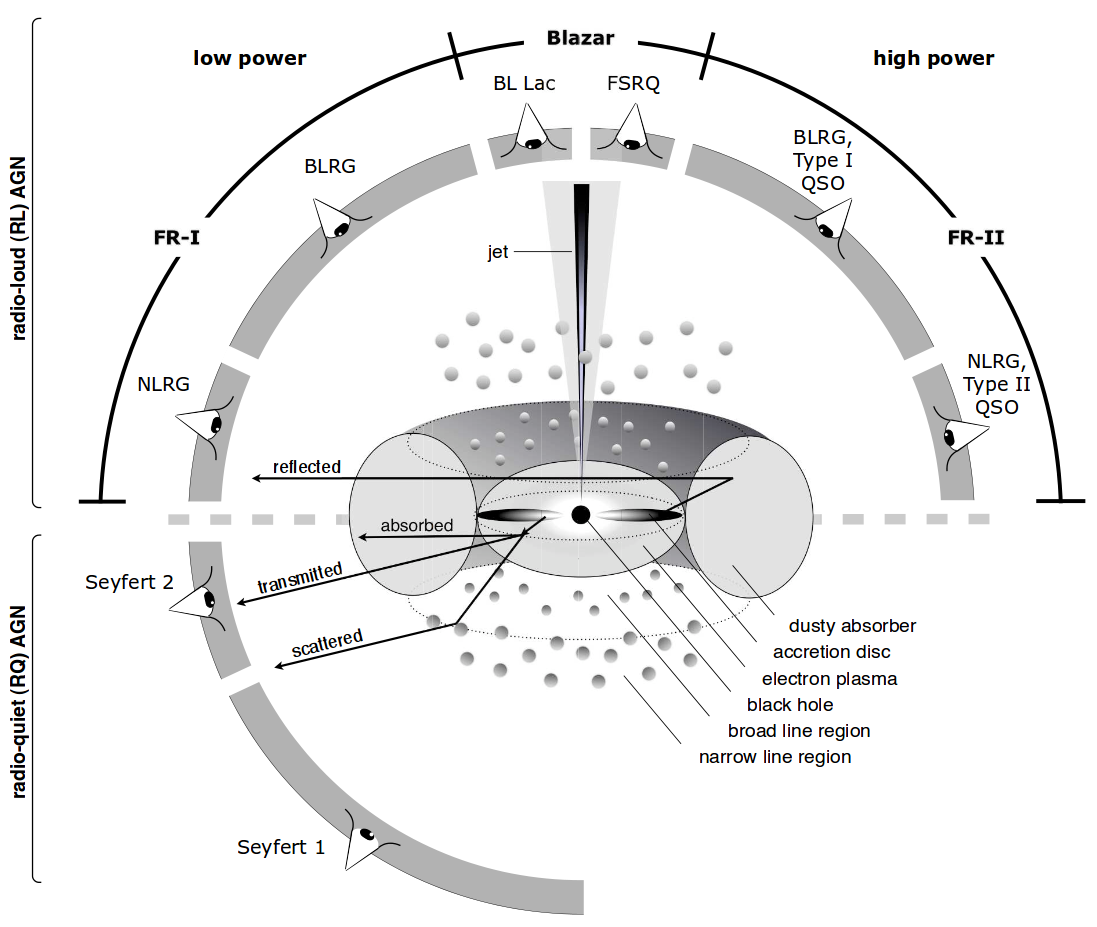
\includegraphics[width=0.8\textwidth]{./Plots/02_Astroteilchenphysik/AGN_Schema.png}
    \caption{Schematische Darstellung einer AGN. Abhängig von der Radioemission und dem Blickwinkel werden die einzelnen AGN-Typen voneinander unterschieden.
    Im Inneren befindet sich ein supermassives schwarzes Loch, welches von einer Akkretionsscheibe umgeben ist. 
    Diese wird wiederum von einem Staubtorus umschlossen.
    Aus dem Zentrum werden zwei entgegengesetzte Jets emittiert.\cite{AGNSchema}}
    \label{AGN_Bild}
\end{figure}

Wie in \autoref{AGN_Bild} zu sehen ist, befindet sich im Zentrum jeder AGN ein supermassives schwarzes Loch, welches Materie akkretiert und eine Akkretionsscheibe formt.
Oberhalb der Scheibe befinden sich Wolken, die mit schneller Geschwindigkeit rotieren und Emissionslinien fabrizieren. Diese Region wird Broad Line Region (BLR) genannt.
Wolken die mit einem größeren Abstand um das schwarze Loch kreisen produzieren die narrow lines und werden Narrow Line Region genannt.
Die BLR und die zentrale Region sind von einem Staubtorus umgeben.
Senkrecht zur Scheibe werden zwei Jets in entgegengesetzte Richtungen emittiert.\cite{Weekes}

\subsection{Klassifikation}
Nach Urry und Padovani\cite{Urry_Padovani} werden AGNs in radiolaute und radioleise Vertreter unterteilt. 
Diese werden dann wieder gemäß ihrer Ausrichtung zur Sichtlinie des Beobachters weiter klassifiziert.
Für eine genauere Informationen siehe \cite{Urry_Padovani}.
Gemäß dieser Klassifikation werden nun Blazare betrachtet.
Bei diesem AGN-Typ handelt es sich um radiolaute Quellen und der Beobachter guckt in den Jet. 
Blazare können in allen Wellenlängen beobachtet werden, d.h. über die volle Breite des elektromagnetischen Spektrums, was ca. 19 Dekaden in der Energie entspricht.
Sie zeichnen sich durch ihre hohe Luminosität im Gammawellenlängenbereich und große Variabilität in allen Wellenlängen aus.
Des Weiteren können starke Korrelationen zwischen den Wellenlängen beobachtet werden.\cite{Weekes}

\subsection{Spektrale Energieverteilung}
Die spektrale Energieverteilung [Spectral Energy Distribution (SED)] beschreibt die Emission einer Quelle aufgeteilt nach den verschiedenen Wellenlängen.
Die SEDs von Blazaren besitzen eine charakteristische 2-huppelige Struktur.
Bei sehr hochenergetischen Blazaren, wie Mrk 421 und Mrk 501 befindet sich der erste Peak bei Röntgenenergien und der zweite Peak bei ca. (10-250)$\si{GeV}$.
Beide Peaks sind vergleichbar hoch.\cite{Weekes}


\subsection{Variabilität}
Blazare haben charakteristische Variabilitäten zwischen einigen Minuten und Jahren.
Die erste Detektion eines Flares, also eines außergewöhnlichen Flussanstiegs, in der VHE-Emission einer AGN fand 1994 statt:
Whipple beobachtete einen Flussanstieg von Mrk421 auf das 10fache.\cite{Weekes}\cite{Mrk421_Outburst}

\subsection{Multiwellenlängenbeobachtungen}
Die simultane Beobachtung einer Quelle mit mehreren Teleskopen zur genauen Überwachung der Aktivität in allen Wellenlängen wird Multiwellenlängenbeobachtung (MWL-Beobachtung) genannt. 
Diese Beobachtungen dienen z.B. dazu, die Beschleunigungs-Mechanismen in den Quellen zu verstehen.
Es können Korrelationen der Flüsse in verschiedenen Wellenlängen untersucht werden.
Die erste MWL-Kampagne wurde 1995 organisiert; Ziel war die Quelle Mrk421.\cite{Weekes}

\subsection{Modelle für hochenergetische Gamma-Emission}
Es existieren zwei grundsätzlich verschiedene Ansätze um die hochenergetische Gammaemission zu erklären.
Dies sind zum einen leptonische Modelle und zum anderen hadronische Modelle.
Im Folgenden werden zuerst zwei mögliche leptonische Modelle und anschließend ein hadronisches Modell vorgestellt.

\subsubsection{Leptonische Modelle}
Die Spektrale Energieverteilung (SED) gibt Hinweise auf die Strahlungsmechanismen, die im Inneren eines Jets vonstatten gehen könnten.
Im Inneren eines Jets werden Elektronen durch Schocks beschleunigt. 
Diese Schocks entstehen durch Materie-Ansammlungen, die den Jet mit verschiedenen Geschwindigkeiten durchlaufen.
Die beschleunigten Elektronen verlieren ihre Energie durch Synchrotronstrahlung im Magnetfeld des Jets und produzieren den Synchrotronpeak in der SED.
Die Position dieses Peaks wird durch die Effizient der Schockbeschleunigung und der Cooling-Prozesse, d.h. der Energieverluste bestimmt. 
Im Folgenden werden zwei verschiedene leptonische Modelle vorgestellt.\cite{Weekes}

\subparagraph{SSC}
Im Synchrotron-Selbst-Compton-Modell werden die in Synchrotron-Prozessen abgestrahlten Photonen zu hohen Energien geboostet, die nahe an den Elektronenergien sind.
Im Thomson-Regime können Photonenergien von $E_{\gamma}\approx \gamma^2 h \nu$ und im Klein-Nishine-Regima $E_{\gamma}\approx \gamma m_e c^2$ erreicht werden.\cite{Weekes}

\subparagraph{External Radiation Compton}
Im External-Radiation-Compton-Modell werden sogenannte Saat-Photonen benötigt, die dann invers Compton gestreut werden.
Diese Saat-Photonen werden außerhalb des Jets produziert, z.B. in der Akkretionsscheibe.\cite{Weekes}

\subsection{Hadronische Modelle}
In den Protonmodellen werden die Gamma-Photonen in proton-induzierten Kaskaden produziert. 
Ziel dieser Modelle ist es, zwei Phänome gleichzeitig zu erklären: 
Das sind zum Einen die Produktion von VHE-Gammastrahlung in AGNs und zum Anderen der Ursprung der extragalaktischen kosmischen Strahlung mit Energien von $10^{20}\,\si{eV}$.
Die sehr hochenergetische Gammastrahlung entsteht durch beschleunigte Protonen im Jet mit Energien von bis zu $10^{18}\,\si{eV}$, die dann mit energieärmeren Photonen wechselwirken und Pionen produzieren.
Die erzeugten Pionen zerfallen und lösen dann eine Kaskade aus.
In manchen Modellen wird die Gammastrahlung als Synchrotronstrahlung von sehr energiereichen Protonen emittiert.
Das Problem der hadronischen Modelle ist, dass kurze Zeitvariabilitäten nicht erklärt werden können, da dafür ein sehr schnelles Cooling der Protonen nötig wäre. 
Durch Synchrotronstrahlung können die Protonen nicht schnell genug abgebremst werden.
Kollisionen mit Photonen oder Ionen im Jet wären eine bessere Erklärung.\cite{Weekes}

In jedem Fall können hadronische Modell erst dann als richtig angenommen werden, wenn ein Neutrinofluss, resultierend aus dem Pion-Zerfall detektiert wird.\cite{Weekes}




\section{Markarian 421}
\label{sec:Mrk421}

\begin{figure}
    \centering
    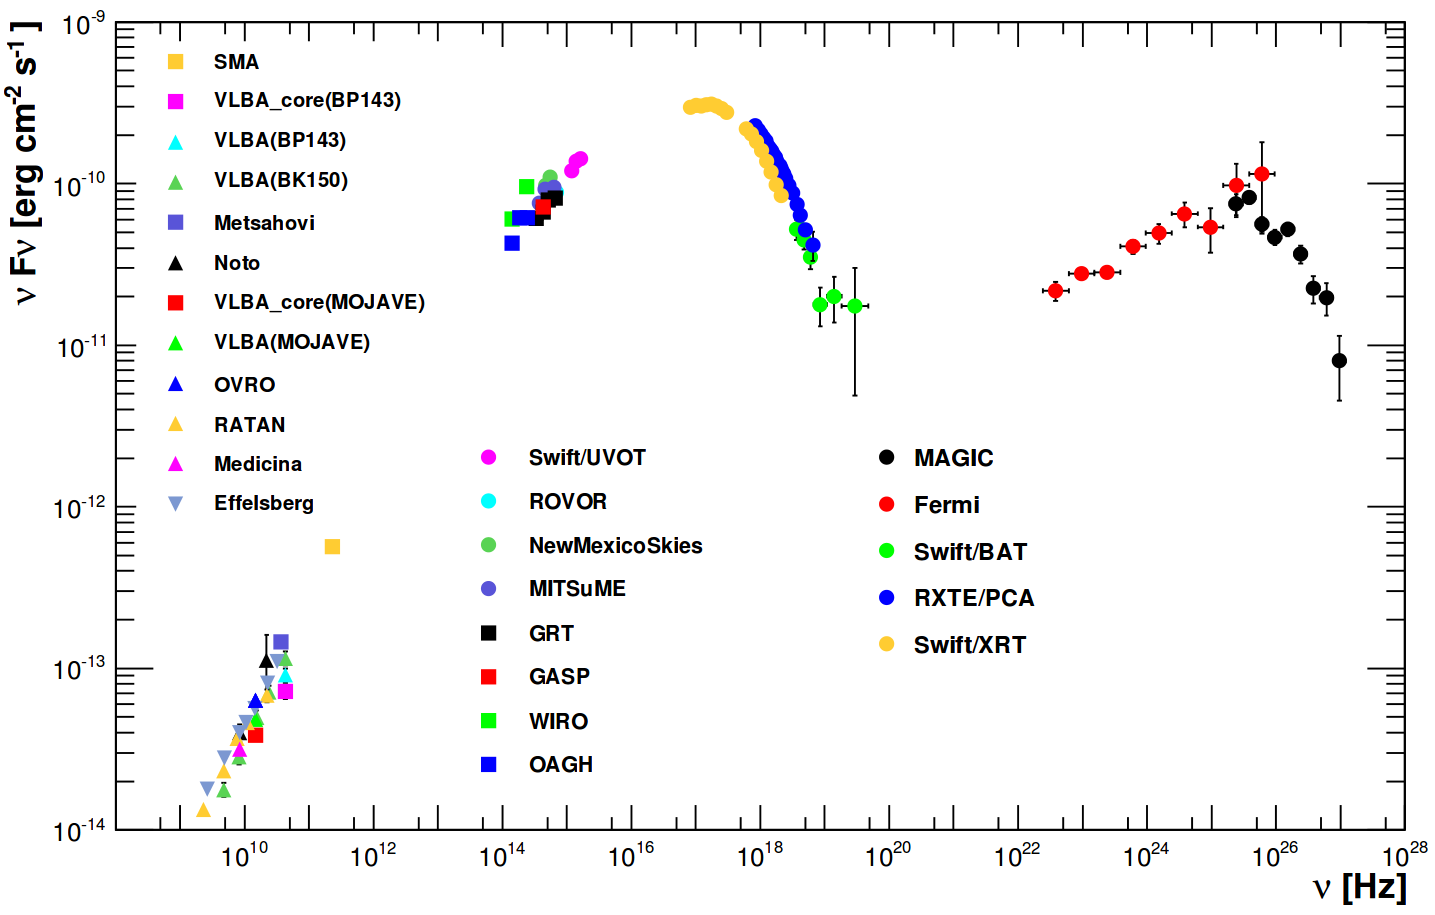
\includegraphics[width=0.8\textwidth]{./Plots/02_Astroteilchenphysik/SED_Mrk421.png}
    \caption{Die Graphik zeigt die SED von Mrk 421. Die für Blazare typische doppelhöckrige Struktur ist erkennbar. 
     Des Weiteren ist zu sehen, dass das Maximum des niederenergetischen und des hochenergetischen Huppels einen ähnlichen Fluss aufweist.\cite{Mrk421_SED}}
    \label{Mrk_SED}
\end{figure}

Die AGN Markarian 421 (Mrk 421) (RA=$11^h 4^m 27,31^s$, Dec=$38°12' 31,8''$) ist eine der hellsten extragalaktischen Quellen im Röntgen- und TeV-Licht und wird dem Typ High Synchrotron Peaked BL Lac zugeordnet.
Sie besitzt eine Rotverschiebung von z=0,0031 und ist damit die nächste Quelle im TeV-Energiebereich.
Neben Mrk 501 ist sie auch die am besten untersuchte Quelle.
Die Quelle ist sehr variabel; so wurde z.B. schon eine Verdopplung des Flusses in $\SI{15}{min}$ beobachtet.
%Es wurden Variationen im Fluss von mehr als einer Ordnung in der Magnitude beobachtet und eine Verdopplung des Flusses in 15min.
Während eines Flares konnte auch eine Änderung in der Steigung des Spektrums beobachtet werden.
In MWL-Kampagnen wurden auch Korrelationen von verschiedenen Wellenlängen beobachtet.
Die charakteristische doppelhöckrige Struktur in der SED ist ebenfalls erkennbar, wobei der erste Peak bei keV-Energien und der zweite bei GeV-TeV-Energien zu erkennen ist (siehe \autoref{Mrk_SED}). 
Mit Hilfe des SSC-Modells kann die Form der SED gut beschrieben werden, wobei hadronische Modelle trotzdem nicht auszuschließen sind.
Die ersten Beobachtungen von MAGIC im Winter 2004/2005 und im Frühling 2005 beinhalten Observationen von Mrk 421.
Eine Multiwellenlängenkampagne von der Quelle hat auch, während die Quelle in einem nicht aktiven Zustand war, Variabilitäten beobachtet und eine Korrelation zwischen VHE und Röntgenstrahlung destgestellt \cite{MWL2009}.\cite{Weekes}